\documentclass[shortpres,usenames,dvipsnames]{beamer}
\usetheme{CambridgeUS}

% Depending on build configuration, one of these packages will
% enable unicode
\usepackage[utf8]{inputenc}
\usepackage{fontspec}
%\usepackage{anyfontsize}		%TODO: Who uses this package???? -> Remove
\usepackage{listings}

%Images
\usepackage{graphicx, svg}
\usepackage{caption}

\usepackage{subfig}
\usepackage{multicol}
\usepackage{color}
\usepackage{pgfplots}
\usepackage{xmpmulti}
\usepackage{verbatim}

%Tikz
\usepackage{tikz}


\usepackage{algorithm,algpseudocode}  %for algorithm environmenstacle in the bathymetry to show the effect of the soruce terms in 2D.t

\setbeamertemplate{footline}
{
	\leavevmode%
	\hbox{%
		\begin{beamercolorbox}[wd=.333333\paperwidth,ht=2.25ex,dp=1ex,center]{author in head/foot}%
			\usebeamerfont{author in head/foot}\insertshortauthor%~~\beamer@ifempty{\insertshortinstitute}{}{(\insertshortinstitute)}
		\end{beamercolorbox}%
		\begin{beamercolorbox}[wd=.333333\paperwidth,ht=2.25ex,dp=1ex,center]{title in head/foot}%
			\usebeamerfont{title in head/foot}\insertshorttitle
		\end{beamercolorbox}%
		\begin{beamercolorbox}[wd=.333333\paperwidth,ht=2.25ex,dp=1ex,right]{date in head/foot}%
			\usebeamerfont{date in head/foot}\insertshortdate{}\hspace*{2em}
			\insertframenumber{} / \inserttotalframenumber\hspace*{2ex}
	\end{beamercolorbox}}%
	\vskip0pt%
}\part{title}
\beamertemplatenavigationsymbolsempty


%color specification---------------------------------------------------------------
\definecolor{TUMblue}{rgb}{0.00, 0.40, 0.74}
\definecolor{TUMgray}{rgb}{0.85, 0.85, 0.86}
\definecolor{TUMpantone285C}{rgb}{0.00, 0.45, 0.81}
\definecolor{lightblue}{rgb}{0.7529,0.8118,0.9333}

\setbeamercolor{block title}{fg=white, bg=TUMpantone285C}
\setbeamercolor{block body}{bg=lightblue}
\setbeamertemplate{blocks}[rounded][shadow=true]
%----------------------------------------------------------------------------------

\setbeamercolor{frametitle}{fg=TUMblue, bg=white}
\setbeamercolor{palette primary}{fg=TUMblue,bg=TUMgray}
\setbeamercolor{palette secondary}{use=palette primary,fg=TUMblue,bg=white}
\setbeamercolor{palette tertiary}{use=palette primary,fg=white, bg=TUMblue}
\setbeamercolor{palette quaternary}{use=palette primary,fg=white,bg=TUMpantone285C}


\setbeamercolor{title}{bg=white,fg=TUMblue}
\setbeamercolor{item projected}{use=item,fg=black,bg = lightblue}
\setbeamercolor{block title}{fg=black, bg=lightblue}
\setbeamercolor{block body}{bg=white}
\setbeamertemplate{blocks}[rounded][shadow=true]
%----------------------------------------------------------------------------------


%############### Self defined commands ##############################
\newcommand{\imgvoffset}{-20pt}
\newcommand{\texthoffset}{20pt}
\newcommand{\imgfullscale}{0.75}
\newcommand{\imgcolscale}{0.9}

\captionsetup[subfigure]{labelformat=empty}		%Disable enumeration of subfigures
%####################################################################

%############### Title information ###############
\title[{Tsunami simulation}]{Assignment 3}
\author[Bellamy, Honal, Wieser]{Gruppe 03\\George Bellamy, Christoph Honal, Felix Wieser\\\vspace{10pt}{\small Bachelorpraktikum}}
\institute[TU M\"unchen]{Technical University of Munich}
\date{5. December 2017}
%#################################################

%############### Tikz picture configuration ###############
\newcommand{\pgfglobalscale}{0.7}
\newcommand{\pgfglobalheadervspace}{\vspace{5pt}\\}
%##########################################################

\lstset{escapeinside={<@}{@>}}

\begin{document}
\maketitle

\begin{frame}{Overview}
	\begin{figure}
		\subfloat[HPC]{\includegraphics[clip,width=0.3\linewidth]
			{img/lrz.png}}
		\hspace{10pt}
		\subfloat[Coarse computation]{
\includegraphics[clip,width=0.3\linewidth]
			{img/dummy_image.jpg}}
		\hspace{40pt}
		\subfloat[Project]{
\includegraphics[clip,width=0.3\linewidth]
			{img/dummy_image.jpg}}
	\end{figure}
\end{frame}

\begin{frame}[fragile]{HPC: Performance analysis (Overview)}
	Analysis overview
	\begin{itemize}
		\item HPC $\leftrightarrow$ PC
		\item \verb|GCC| $\leftrightarrow$ Intel
		\item OpenMP: Basic \verb|for| parallelisation
		\item OpenMP: \verb|assert|, thread workload optimisation, \dots
	\end{itemize}
\end{frame}

\begin{frame}{HPC: Performance analysis (HPC $\leftrightarrow$ PC)}
	%TODO: Add correct data
	\centering
	Computation time analysis\pgfglobalheadervspace
	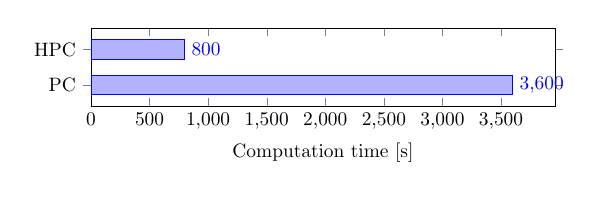
\begin{tikzpicture}[scale=\pgfglobalscale]
		\begin{axis}[
			xbar, xmin=0,
			width=10cm, height=3cm, enlarge y limits=0.6,
			xlabel={Computation time [s]},
			symbolic y coords={PC,HPC},
			ytick=data,
			nodes near coords, nodes near coords align={horizontal},
		]
			\addplot coordinates {(3600,PC) (800,HPC)};
		\end{axis}
	\end{tikzpicture}
	
	Impact on performance\pgfglobalheadervspace
	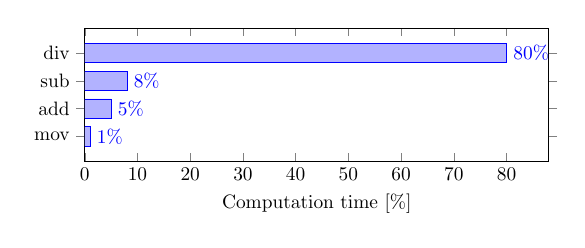
\begin{tikzpicture}[scale=\pgfglobalscale]
		\begin{axis}[
			xbar, xmin=0,
			width=10cm, height=4cm, enlarge y limits=0.3,
			xlabel={Computation time [\%]},
			symbolic y coords={mov, add, sub, div},
			ytick=data,
			nodes near coords, nodes near coords align={horizontal},
			nodes near coords=\pgfmathprintnumber{\pgfplotspointmeta}\%,
		]
			\addplot coordinates {(1,mov) (5,add) (8,sub) (80,div)};
		\end{axis}
	\end{tikzpicture}
	
	Result
	\begin{itemize}
		\item result 1
	\end{itemize}
\end{frame}

\begin{frame}{GCC $\leftrightarrow$ Intel}
	\centering
	Computation time analysis\pgfglobalheadervspace
	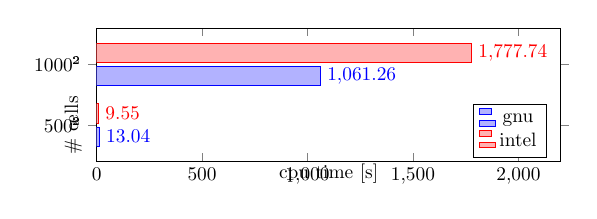
\begin{tikzpicture}[scale=\pgfglobalscale]
	\begin{axis}[
	xbar, xmin=0, xmax=2200,
	width=10cm, height=4cm, enlarge y limits=0.6,
	xlabel={cpu time [s]},
	x label style={at={(axis description cs:0.5,-0.22)}, anchor=south},
	x tick label style={rotate=-45},
	symbolic y coords={500²,1000²},
	ytick=data,
	ylabel=\# cells,
	y label style={at={(axis description cs:-0.05,0.0)},anchor=west},
	x tick label style={rotate=45},
	nodes near coords, nodes near coords align={horizontal},
	legend pos=south east,
	]
	\addplot coordinates {(13.04,500²) (1061.26,1000²)};
	\addplot coordinates {(9.55,500²) (1777.74,1000²)};
	\legend{gnu,intel}
	\end{axis}
	\end{tikzpicture}
	\newline
	{\tiny Runs were performed with 28 threads}
	
	Impact on performance\pgfglobalheadervspace
	%TODO: Implement content
	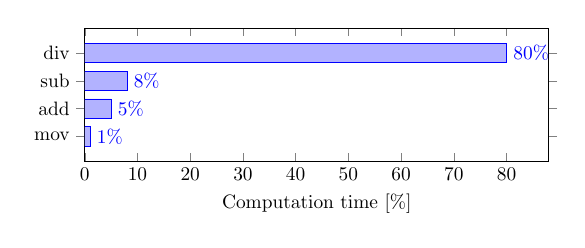
\begin{tikzpicture}[scale=\pgfglobalscale]
	\begin{axis}[
	xbar, xmin=0,
	width=10cm, height=4cm, enlarge y limits=0.3,
	xlabel={Computation time [\%]},
	symbolic y coords={mov, add, sub, div},
	ytick=data,
	nodes near coords, nodes near coords align={horizontal},
	nodes near coords=\pgfmathprintnumber{\pgfplotspointmeta}\%,
	]
	\addplot coordinates {(1,mov) (5,add) (8,sub) (80,div)};
	\end{axis}
	\end{tikzpicture}
	
	Result
	\begin{itemize}
		\item result 1
	\end{itemize}
\end{frame}

\begin{frame}{HPC: OpenMP}
	Questions to answer:
	\begin{itemize}
		\item Run time analysis
		\item Which loop should be parallelized in a two-dimensional domain?
		\item Comparison of scheduling strategies
	\end{itemize}
\end{frame}

\begin{frame}[containsverbatim]{OpenMP: Basic for parallelisation}
	\begin{multicols}{2}
		\begin{lstlisting}[
			language=C++,
			basicstyle=\tiny, numbers=left, stepnumber=1, keywordstyle=\color{blue}\ttfamily,
			stringstyle=\color{red}\ttfamily,
			commentstyle=\color{ForestGreen}\ttfamily,
			xleftmargin=.04\textwidth, xrightmargin=.2\textwidth,
			tabsize=3,
			gobble=9,
			]
			for(int y = 0; y < numRows(); y++)
			{
				//Parallelisation of inner loop
				<@\texttt{\textcolor{orange}{\#pragma parallel for}}@>
				for(int x = 0; x < numCols(); x++)
				{
					doSomething(x,y);
				}
			}
		\end{lstlisting}
			
		\begin{itemize}
			\item Each thread processes one \begin{verbatim}doSomething(x,y)\end{verbatim}
			\item Many context switches
			\item Short thread lifetime
			\item[$\Rightarrow$] Bad performance 
		\end{itemize}
		
	\columnbreak
	
		\begin{lstlisting}[
			language=C++,
			basicstyle=\tiny, numbers=left, stepnumber=1, keywordstyle=\color{blue}\ttfamily,
			stringstyle=\color{red}\ttfamily,
			commentstyle=\color{ForestGreen}\ttfamily,
			xleftmargin=.04\textwidth, xrightmargin=.2\textwidth,
			tabsize=3,
			gobble=9,
			]
			//Parallelisation of outer loop
			<@\texttt{\textcolor{orange}{\#pragma parallel for}}@>
			for(int y = 0; y < numRows(); y++)
			{
				for(int x = 0; x < numCols(); x++)
				{
					doSomething(x,y);
				}
			}
		\end{lstlisting}
		
		\begin{itemize}
			\item Each thread executes one row
			\item Less context switches
			\item Increased thread lifetime
			\item[$\Rightarrow$] Better performance
		\end{itemize}
	\end{multicols}
\end{frame}

\begin{frame}{OpenMP: Advanced parallelisation}
	%TODO: Implement content
	\centering
	Computation time analysis\pgfglobalheadervspace
	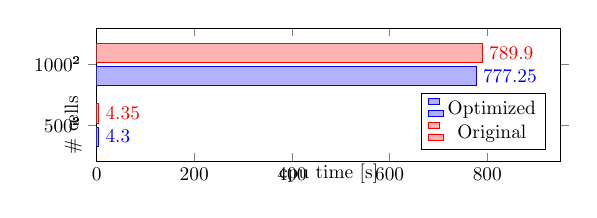
\begin{tikzpicture}[scale=\pgfglobalscale]
	\begin{axis}[
	xbar, xmin=0, xmax=950,
	width=10cm, height=4cm, enlarge y limits=0.6,
	xlabel={cpu time [s]},
	x label style={at={(axis description cs:0.5,-0.22)}, anchor=south},
	x tick label style={rotate=0},
	symbolic y coords={500²,1000²},
	ytick=data,
	ylabel=\# cells,
	y label style={at={(axis description cs:-0.05,0.0)},anchor=west},
	nodes near coords, nodes near coords align={horizontal},
	legend style={at={(0.7,0.3)},anchor=west},
	]
	\addplot coordinates {(4.30,500²) (777.25,1000²)};
	\addplot coordinates {(4.35,500²) (789.90,1000²)};
	\legend{Optimized,Original}
	\end{axis}
	\end{tikzpicture}
	\newline
	{\tiny 56 threads, gnu compiler}
	
	Impact on performance\pgfglobalheadervspace
	%TODO: Implement content
	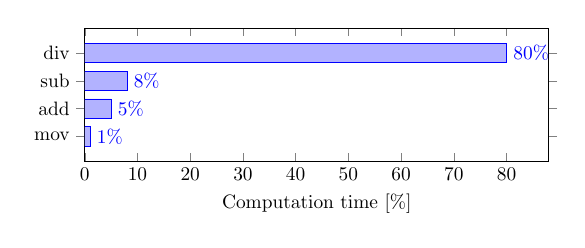
\begin{tikzpicture}[scale=\pgfglobalscale]
	\begin{axis}[
	xbar, xmin=0,
	width=10cm, height=4cm, enlarge y limits=0.3,
	xlabel={Computation time [\%]},
	symbolic y coords={mov, add, sub, div},
	ytick=data,
	nodes near coords, nodes near coords align={horizontal},
	nodes near coords=\pgfmathprintnumber{\pgfplotspointmeta}\%,
	]
	\addplot coordinates {(1,mov) (5,add) (8,sub) (80,div)};
	\end{axis}
	\end{tikzpicture}
	
	Result
	\begin{itemize}
		\item result 1
	\end{itemize}
\end{frame}

\begin{frame}{Coarse computation}
	\begin{multicols}{2}
		Features
		\begin{itemize}
			\item List
			\item of
			\item key
			\item features
		\end{itemize}
	\columnbreak
		 Bild
	\end{multicols}
	
\end{frame}

\begin{frame}{Project}
	Development of a graphical data analyzer
	\begin{itemize}
		\item Standalone visualization of the SWE simulation output
		\item Analysis functionality
		\begin{itemize}
			\item Cell data extraction and visualization over time
			\item Cross-section visualization
			\item Coastal damage assessment (max. wave height and speed)
		\end{itemize}
		\item Data export
		\begin{itemize}
			\item Images
			\item Graphs (i.e. cross-sections)
			\item Video
		\end{itemize}
	\end{itemize}
\end{frame}

\begin{frame}{}
	\begin{figure}
		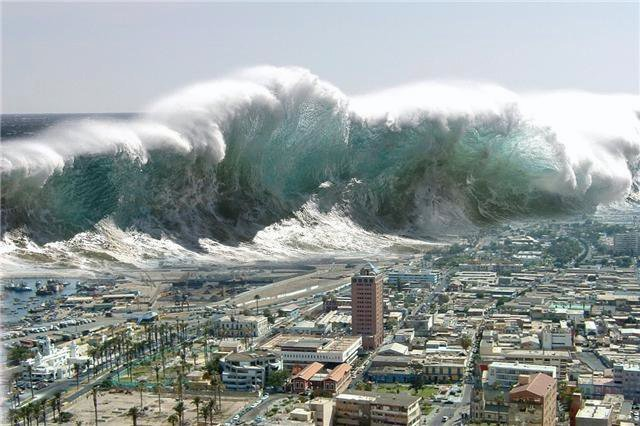
\includegraphics[clip, width=\imgfullscale\linewidth]{img/tsunami.jpg}
	\end{figure}
	\centering
	Thank you for your attention
	\\
	\vfill
	\flushleft
	{\fontsize{5}{5} \selectfont http://userscontent2.emaze.com/images/88c09d66-4283-49c0-9f80-9eb8fd05e30f/16101782-ea98-4b06-b114-4637be705926.jpg}
\end{frame}
\end{document}